\chapter{Case Study on Resource-centric Organizational Modeling}
\label{chap:casestudy}

%of the system: Class diagrams (components), ER, algorithms if there are any
%%Presentation of the functioning system and culmination of the work.
%%Analysis of the work as well as a comparison with the state of the art
In this chapter, we provide architecture of the functioning system as a first section. The section provides, implementation details along with the reason for making certain implementation decisions. The final section validates the system by analyzing the work the validating it with the proposed approach. This section also has some screen results as it helps in validating the functioning of the system as well.

%%%%%%%%%%%%%%%%%%%%%%%%%%%%%%%%%%%%%%%%%%%%%%%%%%%%%%%%%%%%%%%%%%%%%%%%%
\section{Architecture of the Functioning System}
\label{sec:architectureofthefunctioningsystem}
%%%%%%%%%%%%%%%%%%%%%%%%%%%%%%%%%%%%%%%%%%%%%%%%%%%%%%%%%%%%%%%%%%%%%%%%%

User interface URL navigation of the functioning system is provided in the Figure \ref{fig:UIArchitecture}


\begin{figure}
	\centering
	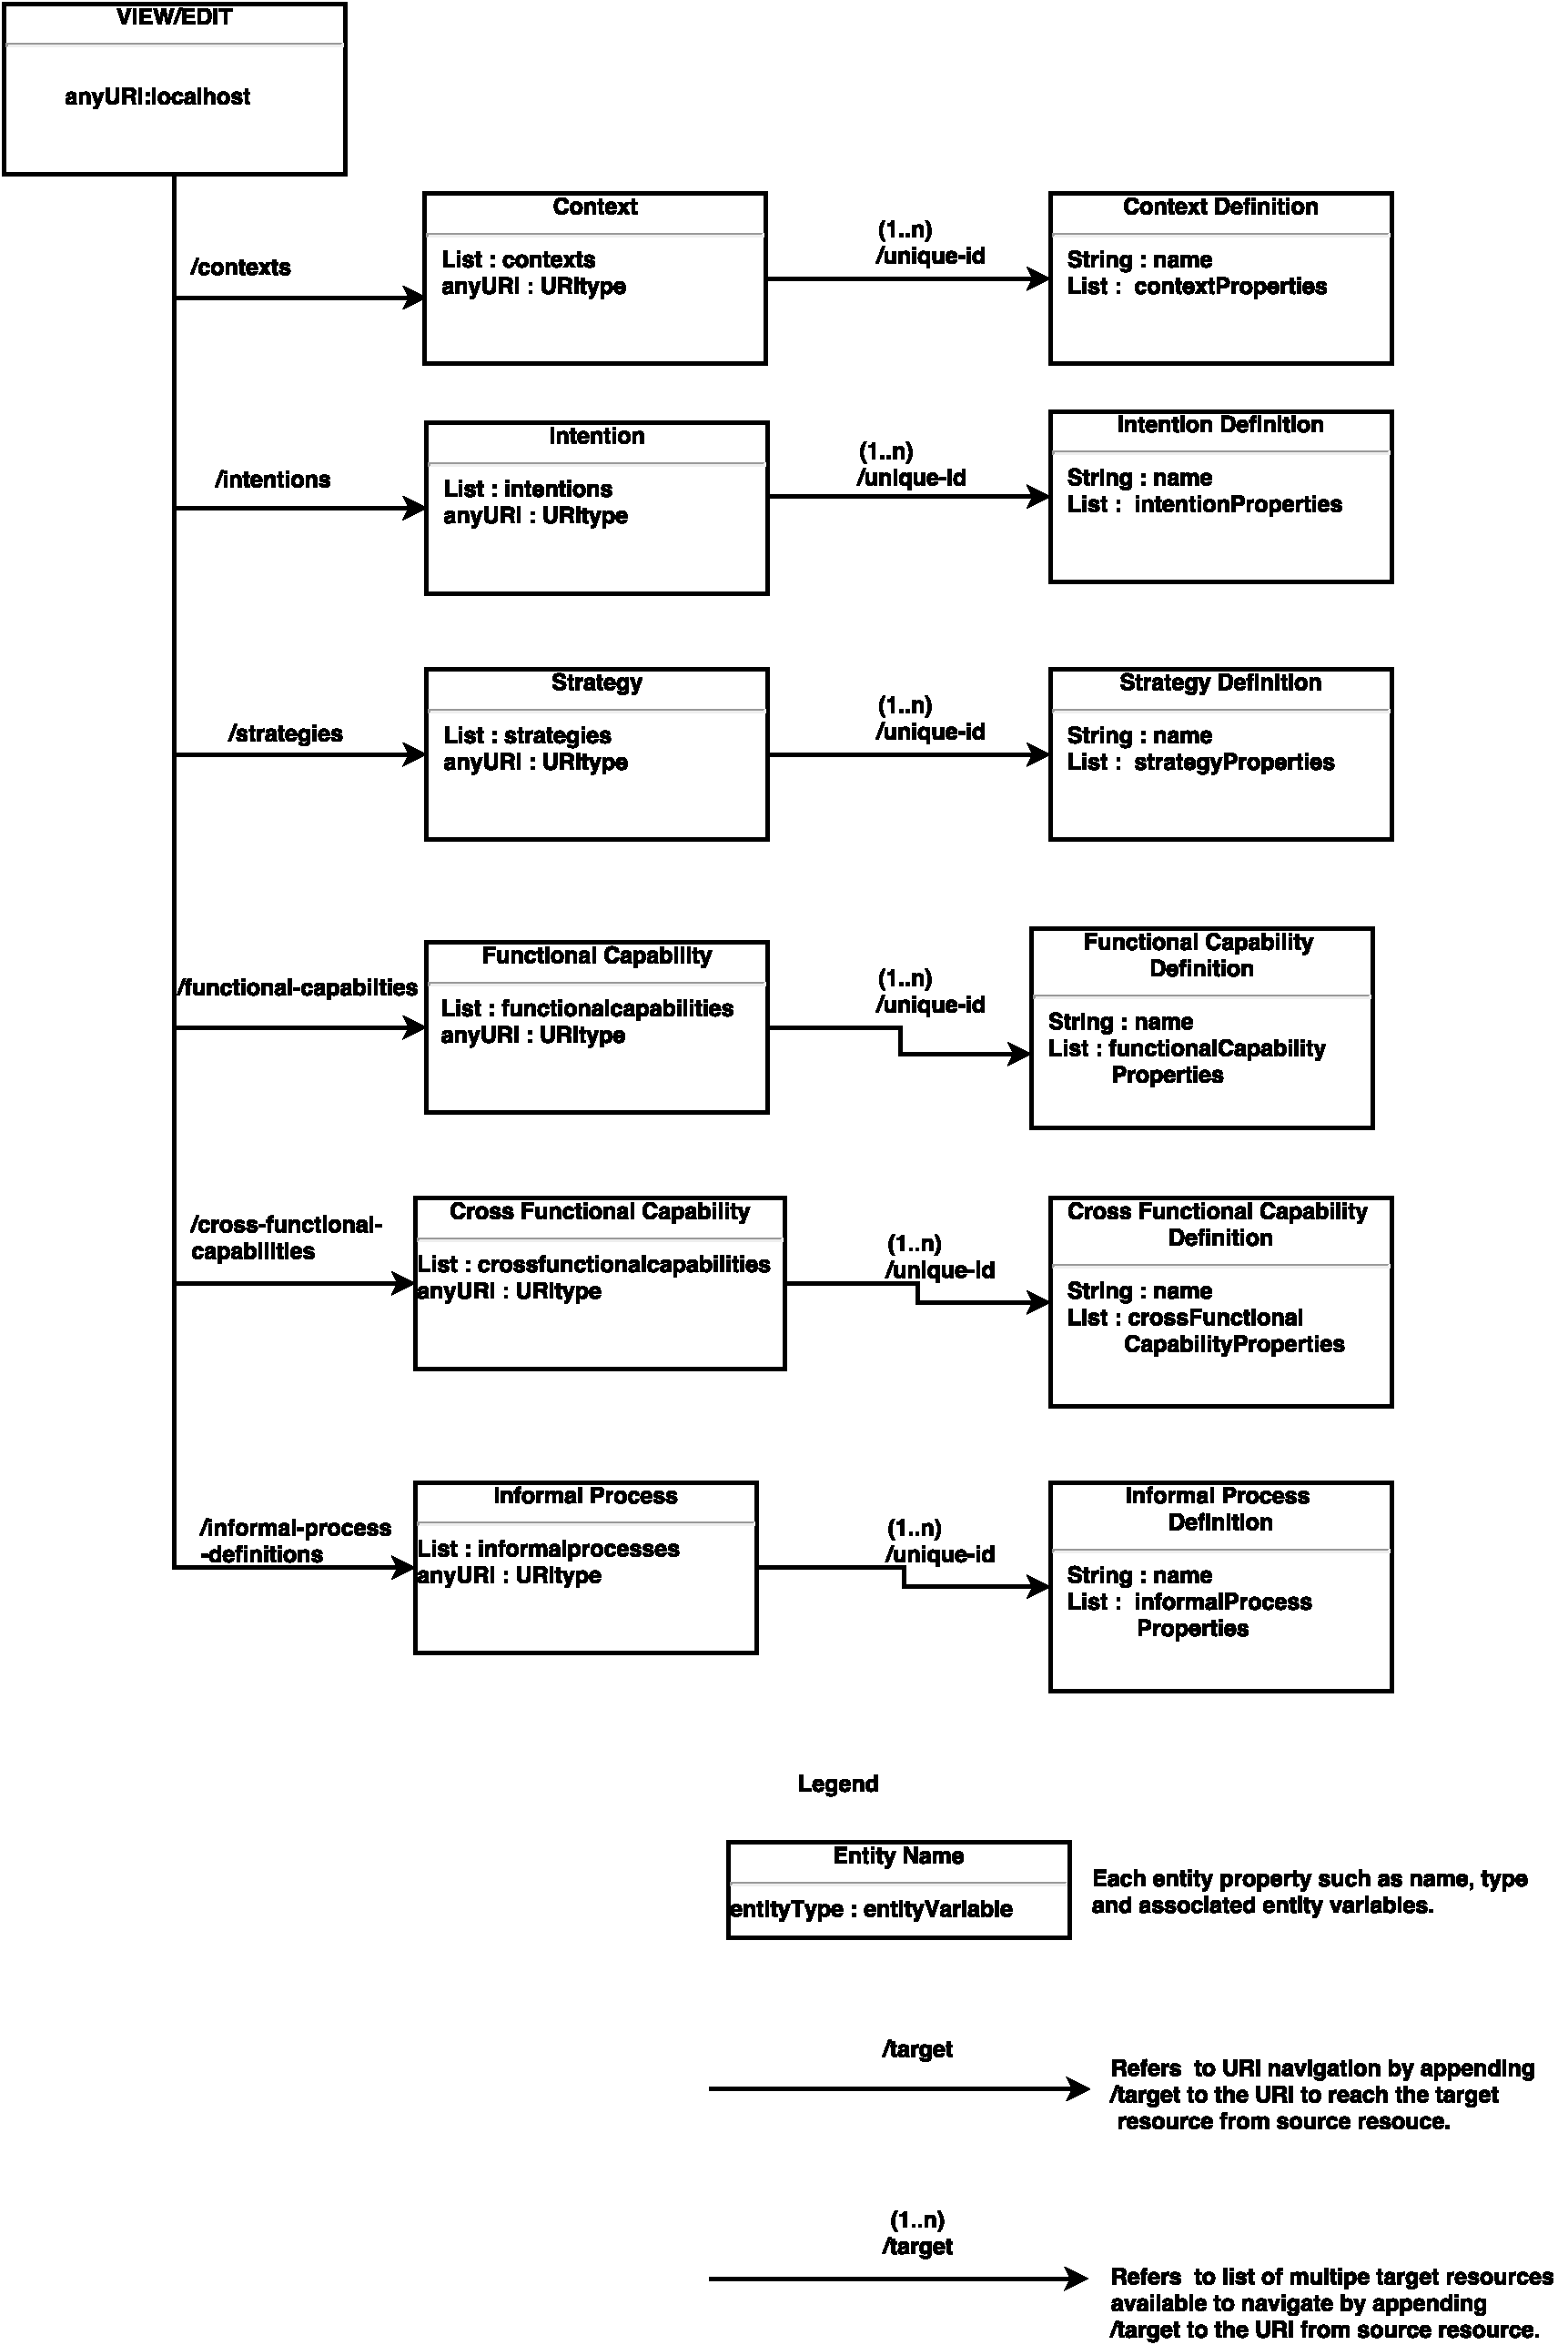
\includegraphics [width= \textwidth]{UIArchitecture.pdf}
	\caption{User interface URL navigation of the functioning system}
	\label{fig:UIArchitecture}
\end{figure}



%%%%%%%%%%%%%%%%%%%%%%%%%%%%%%%%%%%%%%%%%%%%%%%%%%%%%%%%%%%%%%%%%%%%%%%%%
\section{A Concrete View of Entity Types}
\label{sec:realization}
%%%%%%%%%%%%%%%%%%%%%%%%%%%%%%%%%%%%%%%%%%%%%%%%%%%%%%%%%%%%%%%%%%%%%%%%%
%how did I implement, technology and frameworks used and why.

 This chapter discusses about how Intention-centric organizational modeling realized as an user interface editor. This also explains the realization of requirements described in Chapter 4. In the first section, we will first discuss the overview of basic concepts and then specify the design components required for the realization of this editor. The next section discusses about how the entity views in particular are realized. The last section covers in detail how individual requirement has been realized through the web editor.




%%%%%%%%%%%%%%%%%%%%%%%%%%%%%%%%%%%%%%%%%%%%%%%%%%%%%%%%%%%%%%%%%%%%%%%%%
\subsection{Realization of Entity Views}
\label{subsec:realofentityviews}
%%%%%%%%%%%%%%%%%%%%%%%%%%%%%%%%%%%%%%%%%%%%%%%%%%%%%%%%%%%%%%%%%%%%%%%%%
The XML Schema Definition of entity type has been provided in \ref{lst:xsdlist}



\begin{Listing}
	\begin{lstlisting}
	<xs:complexType name="tEntityType" abstract="true">
	<xs:complexContent>
	<xs:extension base="tExtensibleElements">
	<xs:sequence>
	<xs:element name="Tags" type="tTags" minOccurs="0"/>
	<xs:element name="DerivedFrom" minOccurs="0">
	<xs:complexType>
	<xs:attribute name="typeRef" type="xs:QName" use="required"/>
	</xs:complexType>
	</xs:element>
	<xs:element name="PropertiesDefinition" minOccurs="0">
	<xs:complexType>
	<xs:attribute name="element" type="xs:QName"/>
	<xs:attribute name="type" type="xs:QName"/>
	</xs:complexType>
	</xs:element>
	</xs:sequence>
	<xs:attribute name="name" type="xs:NCName" use="required"/>
	<xs:attribute name="abstract" type="tBoolean" default="no"/>
	<xs:attribute name="final" type="tBoolean" default="no"/>
	<xs:attribute name="targetNamespace" type="xs:anyURI" use="optional"/>
	</xs:extension>
	</xs:complexContent>
	</xs:complexType>>
	\end{lstlisting}
	\caption{XML Schema Definition of Entity Type}
	\label{lst:xsdlist}
\end{Listing}

%%%%%%%%%%%%%%%%%%%%%%%%%%%%%%%%%%%%%%%%%%%%%%%%%%%%%%%%%%%%%%%%%%%%%%%%%
\subsection{Realization of Organizational Intentions}
%%%%%%%%%%%%%%%%%%%%%%%%%%%%%%%%%%%%%%%%%%%%%%%%%%%%%%%%%%%%%%%%%%%%%%%%%


%%%%%%%%%%%%%%%%%%%%%%%%%%%%%%%%%%%%%%%%%%%%%%%%%%%%%%%%%%%%%%%%%%%%%%%%%
\subsection{Realization of Organizational  Strategies}
%%%%%%%%%%%%%%%%%%%%%%%%%%%%%%%%%%%%%%%%%%%%%%%%%%%%%%%%%%%%%%%%%%%%%%%%%

%%%%%%%%%%%%%%%%%%%%%%%%%%%%%%%%%%%%%%%%%%%%%%%%%%%%%%%%%%%%%%%%%%%%%%%%%
\subsection{Realization of Organizational Capabilities}
%%%%%%%%%%%%%%%%%%%%%%%%%%%%%%%%%%%%%%%%%%%%%%%%%%%%%%%%%%%%%%%%%%%%%%%%%
There are two types of capabilities. Functional capabilities and cross-functional capabilities. Functional capabilities must be associated with instance descriptors. Cross-functional capabilities are capabilities containing multiple functional capabilities. We need to have the ability to add and remove instance descriptors for an entity type, e.g, resource definitions,  informal process definitions, etc. An instance descriptor of a functional capability should refer to a resource definition meaning that a capability is provided by a resource definition. So an instance descriptor of a capability refers to a resource definition and we can manually add and remove resource definitions in general.




%%%%%%%%%%%%%%%%%%%%%%%%%%%%%%%%%%%%%%%%%%%%%%%%%%%%%%%%%%%%%%%%%%%%%%%%%
\subsection{Realization of Organizational Resources}
%%%%%%%%%%%%%%%%%%%%%%%%%%%%%%%%%%%%%%%%%%%%%%%%%%%%%%%%%%%%%%%%%%%%%%%%%
There are two keys, one for tosca repository and one for tosca modeling tool. Tosca repository url refers to winery and the other one refers to topology modeler. This should only contain root contexts and additional suffixes such as service templates in a separate key in default db.Out of these a function should create corresponding url for topology modeling. The topology modeler page of a specific service temple without knowing its id and namespace. This can be composed from different variables: :topology-modeler-url, :tosco-repository-url,:target-namespace, and :id.


\fbox{\begin{minipage}{\textwidth}
		\{topology-modeler-url\}?repositoryURL=\{encoded-tosca-repository-url\}\&ns=\{encoded-target-namepsace\}\&id=\{encoded-id\}\#
	\end{minipage}}
	
		
What important is, at the end editor should have a view that is capable of adding, viewing, deleting and updating models aligned with the XSD schema. In general, separate entities should reference each other but not contain each other. For instance, a strategy containing a goal should use goals id to resolve it but not the actual goal.
	
%%%%%%%%%%%%%%%%%%%%%%%%%%%%%%%%%%%%%%%%%%%%%%%%%%%%%%%%%%%%%%%%%%%%%%%%%
	\subsection{Realization of Organizational Processes}
%%%%%%%%%%%%%%%%%%%%%%%%%%%%%%%%%%%%%%%%%%%%%%%%%%%%%%%%%%%%%%%%%%%%%%%%%
	
	
%%%%%%%%%%%%%%%%%%%%%%%%%%%%%%%%%%%%%%%%%%%%%%%%%%%%%%%%%%%%%%%%%%%%%%%%%
	\subsection{Realization of Informal Process Instances}
%%%%%%%%%%%%%%%%%%%%%%%%%%%%%%%%%%%%%%%%%%%%%%%%%%%%%%%%%%%%%%%%%%%%%%%%%
	Informal process instances are separate entities similar to informal process models. They should be listed on the left side similar to informal process models. When one of the instance is selected by user, its properties should be presented on the right.
	
	
%%%%%%%%%%%%%%%%%%%%%%%%%%%%%%%%%%%%%%%%%%%%%%%%%%%%%%%%%%%%%%%%%%%%%%%%%
\section{Validation}
\label{sec:validation}
%%%%%%%%%%%%%%%%%%%%%%%%%%%%%%%%%%%%%%%%%%%%%%%%%%%%%%%%%%%%%%%%%%%%%%%%%	
This section validates the research objectives discussed in Chapter \ref{chap:introduction} and prototype developed through the approach discussed in Chapter \ref{chap:approach} using the motivating scenario discussed in Chapter \ref{chap:motivatingScenario}.
	
	
%%%%%%%%%%%%%%%%%%%%%%%%%%%%%%%%%%%%%%%%%%%%%%%%%%%%%%%%%%%%%%%%%%%%%%%%%
\subsection{Validation of Research Objectives}
\label{subsec:validationofrequirements}
%%%%%%%%%%%%%%%%%%%%%%%%%%%%%%%%%%%%%%%%%%%%%%%%%%%%%%%%%%%%%%%%%%%%%%%%%
As discussed in Chapter \ref{chap:approach}, the research objectives are satisfied at the design level but their validity can be confirmed only by evaluating the research objectives with some sample scenarios, like the one provided in Chapter \ref{chap:motivatingScenario}.   

\textit{Organizational intentions transparency} (R1): A valid user whose credentials are stored in database is able to login successfully and view the intentions and its associated entities. Hence the research objective R1 is met.

\textit{Organizational intention resource-based cost estimation} (R2): An intention whose cost is unspecified for a sample intention, is calculated by the developed system recursively as mentioned in the Chapter \ref{chap:approach}. Thus the research objective R2 is also met.

\textit{Organizational intention achievability estimation} (R3): Similar to cost calculation, an intention instance whose achievability is not in prior is also estimated by the current functioning system. Hence research objective R3 is satisifed.

\textit{Intention oriented working style} (R4): The users can login and create intention models, strategy models, informal process models etc., through the developed editor. Hence research objective R4 is also met.

\textit{Participative organizational modeling} (R5): Each entity type that can be acquired or instantiated has list of participants with their corresponding privileges. Thus this satisfies the requirements of research objective R5.

\textit{Re-use of organizational knowledge} (R6): The descriptive information about each models can be stored and re-used for next enactments. Hence research objective R6 is also met.
	
%%%%%%%%%%%%%%%%%%%%%%%%%%%%%%%%%%%%%%%%%%%%%%%%%%%%%%%%%%%%%%%%%%%%%%%%%
\section{Validation of Prototype}
\label{sec:validationofprototype}
%%%%%%%%%%%%%%%%%%%%%%%%%%%%%%%%%%%%%%%%%%%%%%%%%%%%%%%%%%%%%%%%%%%%%%%%%
how research objectives are satisfied. 
	%queries and print screens

	

	


